\chapter{Classical Source Detection Algorithms}
\label{ch:classical}

\textit{This chapter introduces the four classical algorithms used as baselines in every
source-detection benchmark: a uniform random guesser, a degree-centrality ranker, the
Jordan Center, and Rumor Centrality. Each method encodes a different hypothesis about
what makes a good source candidate. By studying them carefully --- including their
assumptions, their failure modes, and the concrete arithmetic behind them --- you will
build the intuition needed to understand why graph neural networks are a principled
improvement, and what benchmark bar they must clear.}

% ============================================================
\section{Overview: A Map of Classical Methods}
\label{sec:classical-overview}
% ============================================================

Before we commit to any single algorithm, it helps to see the whole landscape at a
glance. The table below compares the four methods along the dimensions that matter most
for a practitioner: how fast they are, whether they even look at the contact network,
and whether any theoretical guarantee backs up their predictions.

\begin{table}[H]
\centering
\caption{Comparison of the four classical source-detection baselines. $N$ = number of
nodes; $|\mathcal{I}|$ = number of infected nodes; $|E_{\mathcal{I}}|$ = edges in the
infected subgraph. The ``Network required?'' column asks whether the method needs the
contact graph or only the compartment labels.}
\label{tab:classical-overview}
\small
\begin{tabular}{lllcc}
\toprule
\textbf{Method} & \textbf{Complexity} & \textbf{Network required?} &
  \textbf{Uses observation?} & \textbf{Theoretical guarantee?} \\
\midrule
Uniform random guess & $O(1)$          & No  & No  & Yes --- lower bound only \\
Degree centrality    & $O(N + |E|)$    & Yes & No  & No                      \\
Jordan Center        & $O(|\mathcal{I}| + |E_{\mathcal{I}}|)$
                                       & Yes & Yes (topology only) & No     \\
Rumor Centrality     & $O(|\mathcal{I}|)$ & Yes & Yes & Yes --- ML on regular trees \\
\bottomrule
\end{tabular}
\end{table}

\begin{conceptbox}{What Is a ``Baseline'' and Why Do We Need One?}
A \textbf{baseline} is the simplest possible algorithm that is still a valid answer to
the problem. It sets the floor: any serious method must beat it, and the gap between
the baseline and a sophisticated method measures how much we have actually learned.

In source detection, the most natural floor is the \textbf{random guesser}: without any
information, pick a node uniformly at random. If your fancy algorithm cannot consistently
beat this, it has learned nothing from the data.

Baselines also act as sanity checks. If a new GNN model scores below the Jordan Center
on every experiment, something is broken --- not in the Jordan Center, but in the
training procedure, the data pipeline, or the model itself. This is precisely why the
\texttt{main\_eval.py} script in this codebase runs all four baselines automatically on
every dataset, logging the results to Weights \& Biases for side-by-side comparison.
\end{conceptbox}

% ============================================================
\section{Baseline 1: Uniform Random Guess}
\label{sec:uniform}
% ============================================================

\subsection{The Idea}

The uniform random guesser assigns the same probability to every node in the network:

\begin{equation}
  P_{\text{uniform}}(v) = \frac{1}{N} \quad \text{for all } v \in V.
  \label{eq:uniform}
\end{equation}

There is no computation, no network traversal, no comparison to the observation. Every
node is equally likely to be the source. This is the ``I have no idea'' algorithm.

\begin{analogybox}{The Lottery Ticket Drawer}
Imagine $N = 100$ lottery tickets in a hat, each bearing the name of one node. The
uniform guesser draws one ticket without looking. The true source wins the draw with
probability $1/100 = 1\%$. There is no skill involved, no information used.

The value of this analogy is that it makes the expected performance concrete. If you
repeat this lottery over many independent epidemics, the true source will be in the
top-1 prediction exactly $1\%$ of the time. Any method that achieves, say, $12\%$
top-1 accuracy has beaten the lottery by a factor of 12 --- a meaningful improvement.
\end{analogybox}

\subsection{The Rank Score Metric}

Before we can compute the ``expected performance'' of any method, we need to agree on
how performance is measured. This workbook uses two metrics extensively.

\textbf{Rank of the true source.} After running an algorithm, rank all $N$ nodes by
their predicted probability (highest = rank 1). The rank of the true source $s^*$
tells us how far down the list we have to go to find the right answer. Rank 1 means
the algorithm got it right; rank $N$ means the true source was dead last.

\textbf{Rank score.} The rank score converts a raw rank $r$ into a number between 0
and 1 where higher is better:

\begin{equation}
  \text{RankScore}(r) = \frac{1}{r}.
  \label{eq:rank-score}
\end{equation}

A rank of 1 gives a score of 1.0 (perfect). A rank of 10 gives 0.1. A rank of 100
gives 0.01. We average this score over all epidemic runs to get a single summary number.

\begin{mathbox}{Expected Rank Score of the Uniform Baseline}
\textbf{Setup.} There are $N$ candidate nodes. The uniform guesser assigns equal
probability $1/N$ to every node, so ties are broken by random shuffling. The true
source ends up in a uniformly random position among the $N$ slots.

\textbf{Expected rank.} Since each of the $N$ positions is equally likely:
\[
  \mathbb{E}[\text{rank}] = \frac{1 + 2 + \cdots + N}{N} = \frac{N+1}{2}.
\]
For $N = 100$: $\mathbb{E}[\text{rank}] = 50.5$.

\textbf{Expected rank score.} By Jensen's inequality, $\mathbb{E}[1/r] \neq 1/\mathbb{E}[r]$.
The exact value requires summing over all positions:
\[
  \mathbb{E}\!\left[\frac{1}{r}\right]
  = \frac{1}{N} \sum_{r=1}^{N} \frac{1}{r}
  = \frac{H_N}{N},
\]
where $H_N = \sum_{r=1}^{N} 1/r$ is the $N$-th harmonic number.

\medskip
\begin{center}
\small
\begin{tabular}{rrrr}
\toprule
$N$ & $\mathbb{E}[\text{rank}]$ & $H_N$ & $\mathbb{E}[\text{RankScore}]$ \\
\midrule
10   & 5.5  & 2.93  & 0.293 \\
50   & 25.5 & 4.50  & 0.090 \\
100  & 50.5 & 5.19  & 0.052 \\
500  & 250.5 & 6.79 & 0.014 \\
\bottomrule
\end{tabular}
\end{center}

\medskip
\textbf{Interpretation.} For $N = 100$ nodes, a method that achieves a mean rank score
above $0.052$ has beaten the random floor. The uniform baseline defines the minimum bar.

\textbf{Important nuance.} In the codebase, not all $N$ nodes are valid source
candidates: the \texttt{possible} binary mask in \texttt{TSIRData} excludes nodes that
could not have started a large enough outbreak given the observed infection size. The
effective pool is therefore often smaller than $N$, raising the uniform floor.
Specifically, if $N_{\text{eff}}$ nodes are in the \texttt{possible} mask, the uniform
baseline assigns probability $1/N_{\text{eff}}$ to each valid candidate and zero to
the rest.
\end{mathbox}

\subsection{Implementation in the Codebase}

The uniform baseline lives in \texttt{eval/benchmark.py}. It is implemented in three
lines:

\begin{codewalk}{Uniform Baseline --- \texttt{eval/benchmark.py}}
\begin{lstlisting}[language=Python]
def uniform_probabilities(possible):
    """
    Assign equal probability to every candidate node.

    Parameters
    ----------
    possible : np.ndarray of shape (n_runs, n_nodes)
        Binary mask; 1 if the node is a valid source candidate.

    Returns
    -------
    np.ndarray of shape (n_runs, n_nodes)
        Probability distribution: 1/N_eff for valid candidates, 0 otherwise.
    """
    return possible / np.sum(possible, axis=1, keepdims=True)
\end{lstlisting}

\textbf{What this does, step by step.}
\begin{enumerate}
  \item \texttt{possible} is a matrix with one row per epidemic run and one column per
        node. A 1 in position $(r, v)$ means node $v$ is a valid candidate for run $r$.
  \item \texttt{np.sum(possible, axis=1, keepdims=True)} counts how many valid
        candidates there are in each run. This is $N_{\text{eff}}$ per run.
  \item Dividing \texttt{possible} by this count spreads probability uniformly across
        valid candidates, leaving zeros for invalid ones.
\end{enumerate}
The function returns a proper probability distribution (all rows sum to 1).
\end{codewalk}

% ============================================================
\section{Baseline 2: Degree Centrality}
\label{sec:degree}
% ============================================================

\subsection{The Idea and Its Justification}

The degree of a node $v$ in an undirected network is the number of edges incident to it:

\begin{equation}
  \deg(v) = |\{u \in V : (u, v) \in E\}|.
  \label{eq:degree}
\end{equation}

The degree-centrality heuristic ranks nodes by their degree and predicts the
highest-degree node as the most likely source:

\begin{equation}
  \hat{s}_{\text{degree}} = \arg\max_{v \in V} \deg(v).
  \label{eq:degree-heuristic}
\end{equation}

\textbf{Why might this work?} A node with many connections --- a \textbf{hub} ---
contacts more people per unit time than a peripheral node. During an epidemic, a hub
that becomes infected early will, on average, infect more neighbours sooner, producing
a larger and more centrally-located outbreak. If we observe a large outbreak and
try to guess where it started, the hub is a rational first suspect.

\begin{analogybox}{The Well-Connected Person at a Party}
Imagine you arrive at a party where 30 out of 100 guests have already come down with
norovirus. You need to identify Patient Zero. You know nothing about who interacted
with whom during the illness, but you do know the social structure: some people talked
to almost everyone (the extroverts, high degree), and some barely spoke to anyone
(the wallflowers, low degree).

The degree heuristic says: blame the extrovert first. On average, a highly connected
person is more likely to have spread the infection to so many people. This is a
reasonable prior, but it ignores the actual infection pattern. Maybe the wallflower
was the first to get sick, and the extrovert caught it from them.
\end{analogybox}

\subsection{Worked Example on a 5-Node Graph}

\begin{examplebox}{Degree Centrality on a 5-Node Network}
\textbf{Graph.} Five nodes $\{v_1, v_2, v_3, v_4, v_5\}$ with the following edges:
$(v_1, v_2)$, $(v_1, v_3)$, $(v_1, v_4)$, $(v_2, v_3)$, $(v_3, v_5)$.

\begin{center}
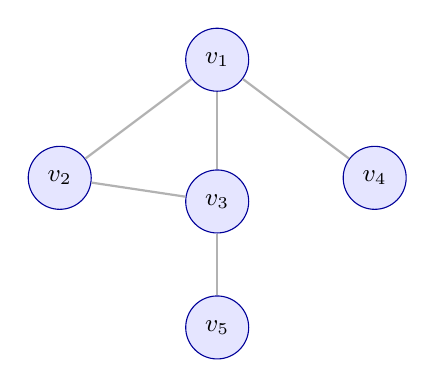
\begin{tikzpicture}[
  nd/.style={circle, draw=blue!60!black, fill=blue!10, minimum size=0.8cm,
             font=\small\bfseries},
  inf/.style={circle, draw=red!60!black, fill=red!15, minimum size=0.8cm,
              font=\small\bfseries},
  edge/.style={thick, gray!60}
]
  \node[nd] (v1) at (0, 0)    {$v_1$};
  \node[nd] (v2) at (-2, -1.5){$v_2$};
  \node[nd] (v3) at (0, -1.8) {$v_3$};
  \node[nd] (v4) at (2, -1.5) {$v_4$};
  \node[nd] (v5) at (0, -3.4) {$v_5$};

  \draw[edge] (v1) -- (v2);
  \draw[edge] (v1) -- (v3);
  \draw[edge] (v1) -- (v4);
  \draw[edge] (v2) -- (v3);
  \draw[edge] (v3) -- (v5);
\end{tikzpicture}
\end{center}

\textbf{Step 1: Compute degrees.}
\begin{center}
\small
\begin{tabular}{lcc}
\toprule
Node & Neighbours & Degree \\
\midrule
$v_1$ & $v_2, v_3, v_4$ & 3 \\
$v_2$ & $v_1, v_3$       & 2 \\
$v_3$ & $v_1, v_2, v_5$  & 3 \\
$v_4$ & $v_1$            & 1 \\
$v_5$ & $v_3$            & 1 \\
\bottomrule
\end{tabular}
\end{center}

\textbf{Step 2: Rank by degree (ties broken randomly).}
$v_1$ and $v_3$ both have degree 3. One is ranked first, the other second.

\textbf{Step 3: The prediction.} The degree heuristic predicts either $v_1$ or $v_3$
as the source (a coin flip between the two).

\textbf{Scenario A: True source is $v_1$.} Degree heuristic is correct 50\% of the
time (when $v_1$ wins the tie-break). Top-2 accuracy is 100\%.

\textbf{Scenario B: True source is $v_4$.} Degree heuristic predicts $v_1$ or $v_3$
(both wrong). The true source $v_4$ has the lowest degree (degree 1). The algorithm
fails completely --- it is farthest from the right answer.

\textbf{Takeaway.} Degree centrality is a useful prior on hub-seeded outbreaks but is
systematically wrong when the true source is peripheral.
\end{examplebox}

\subsection{The Critical Limitation: Blindness to the Observation}

The most important weakness of degree centrality is that it does not look at
\textit{who is actually infected}. Consider two scenarios:

\begin{enumerate}
  \item \textbf{Hub-initiated outbreak.} Node $v_1$ (degree 10) starts the epidemic.
        After $T = 5$ steps, its 10 direct neighbours are all infected. The degree
        heuristic correctly ranks $v_1$ first.

  \item \textbf{Peripheral-node outbreak.} Node $v_{99}$ (degree 1) starts the
        epidemic. By coincidence, it is connected to the hub, which then spreads the
        infection widely. The degree heuristic ranks $v_{99}$ last --- completely wrong.
\end{enumerate}

In both scenarios, the degree heuristic produces the identical ranking. It is
``observation-blind'': the actual pattern of infection carries zero weight in its
prediction.

\begin{keyinsight}{Degree Centrality as a Prior, Not a Likelihood}
In Bayesian language, degree centrality is a \textbf{prior}: it encodes our belief
about which nodes are likely sources \emph{before we observe the epidemic}. On
scale-free networks (where hubs are disproportionately common), this prior is
informative. But a good inference algorithm should update this prior with the
\textbf{likelihood} of the observed infection pattern given each candidate source.

The Jordan Center and Rumor Centrality (sections below) take a first step in this
direction: they ask not just ``who is likely to have started it?'' but ``given the
pattern I see, which node is most consistent with being the origin?''
\end{keyinsight}

% ============================================================
\section{Baseline 3: Jordan Center}
\label{sec:jordan}
% ============================================================

\subsection{Motivation: The Source Is Near the Center}

When a disease starts at node $s$ and spreads outward, the infected subgraph grows
like a ripple in a pond: the source is at the center, and the infection front is at
the periphery. At any observation time $T$, the infected nodes form a connected (or
nearly connected) subgraph, and the source is located somewhere near the geometric
center of that subgraph.

This geometric intuition motivates the \textbf{Jordan Center}: find the node that is
closest to all other infected nodes simultaneously --- the node that minimises the
maximum distance to any other infected node.

\begin{conceptbox}{Key Definitions: Distance, Eccentricity, and Jordan Center}
Let $\mathcal{I} \subseteq V$ denote the set of infected (I or R) nodes at observation
time $T$. Let $G_{\mathcal{I}}$ be the subgraph induced by $\mathcal{I}$.

\medskip
\textbf{Shortest-path distance.} The distance $d(u, v)$ between two nodes $u, v \in
\mathcal{I}$ is the number of edges on the shortest path between them in
$G_{\mathcal{I}}$.

\medskip
\textbf{Eccentricity.} The eccentricity of a node $v \in \mathcal{I}$ is:
\begin{equation}
  \text{ecc}(v) = \max_{u \in \mathcal{I}} d(v, u).
  \label{eq:eccentricity}
\end{equation}
The eccentricity measures how far the most distant infected node is from $v$. A small
eccentricity means $v$ is ``centrally located'' within the infected subgraph.

\medskip
\textbf{Jordan Center.} The Jordan Center is the node (or set of nodes) with minimum
eccentricity within the infected subgraph:
\begin{equation}
  \hat{s}_{\text{Jordan}} = \arg\min_{v \in \mathcal{I}} \text{ecc}(v).
  \label{eq:jordan}
\end{equation}
This is also known as the \textbf{graph center} or \textbf{$1$-center} of the induced
subgraph.
\end{conceptbox}

\subsection{Step-by-Step Example on a 6-Node Infected Subgraph}

\begin{examplebox}{Jordan Center Computation on a 6-Node Subgraph}
\textbf{Setup.} Six infected nodes $\{A, B, C, D, E, F\}$ with edges:
$(A,B)$, $(B,C)$, $(C,D)$, $(C,E)$, $(E,F)$.

\textbf{Graph layout (draw it):}
\begin{center}
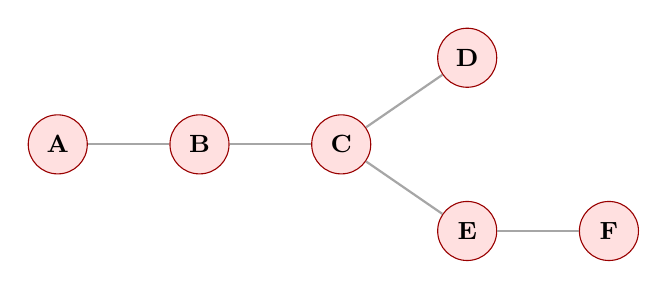
\begin{tikzpicture}[
  nd/.style={circle, draw=red!60!black, fill=red!12, minimum size=0.75cm,
             font=\small\bfseries},
  edge/.style={thick, gray!70}
]
  \node[nd] (A) at (0, 0)   {A};
  \node[nd] (B) at (1.8, 0) {B};
  \node[nd] (C) at (3.6, 0) {C};
  \node[nd] (D) at (5.2, 1.1) {D};
  \node[nd] (E) at (5.2, -1.1){E};
  \node[nd] (F) at (7.0, -1.1){F};

  \draw[edge] (A) -- (B);
  \draw[edge] (B) -- (C);
  \draw[edge] (C) -- (D);
  \draw[edge] (C) -- (E);
  \draw[edge] (E) -- (F);
\end{tikzpicture}
\end{center}

\textbf{Step 1: Compute all pairwise shortest-path distances (BFS from each node).}

\begin{center}
\small
\begin{tabular}{lcccccc}
\toprule
$d(\cdot, \cdot)$ & A & B & C & D & E & F \\
\midrule
A & 0 & 1 & 2 & 3 & 3 & 4 \\
B & 1 & 0 & 1 & 2 & 2 & 3 \\
C & 2 & 1 & 0 & 1 & 1 & 2 \\
D & 3 & 2 & 1 & 0 & 2 & 3 \\
E & 3 & 2 & 1 & 2 & 0 & 1 \\
F & 4 & 3 & 2 & 3 & 1 & 0 \\
\bottomrule
\end{tabular}
\end{center}

\textbf{Step 2: Compute eccentricity for each node} (maximum in its row above).

\begin{center}
\small
\begin{tabular}{lcc}
\toprule
Node & $\max_u d(v, u)$ & Eccentricity \\
\midrule
A & $\max(0,1,2,3,3,4) = 4$ & 4 \\
B & $\max(1,0,1,2,2,3) = 3$ & 3 \\
C & $\max(2,1,0,1,1,2) = 2$ & \textbf{2} \\
D & $\max(3,2,1,0,2,3) = 3$ & 3 \\
E & $\max(3,2,1,2,0,1) = 3$ & 3 \\
F & $\max(4,3,2,3,1,0) = 4$ & 4 \\
\bottomrule
\end{tabular}
\end{center}

\textbf{Step 3: Identify the Jordan Center.}
The minimum eccentricity is 2, achieved uniquely by node $C$.

$\hat{s}_{\text{Jordan}} = C$.

\textbf{Interpretation.} Node $C$ is the most ``central'' node in the infected
subgraph in the sense that even its farthest infected neighbour (nodes $A$ or $F$) is
only 2 hops away. Any other node has at least one infected node at distance 3 or 4.

\textbf{Is the prediction correct?} If the true source is $C$, yes. If the epidemic
actually started at $B$ (which is also fairly central), the Jordan Center gives rank 2
--- still a good prediction.
\end{examplebox}

\subsection{Algorithm Pseudocode}

\begin{codewalk}{Jordan Center --- Pseudocode}
\begin{lstlisting}[language=Python]
from collections import deque

def jordan_center(infected_nodes: list[int],
                  adjacency: dict[int, list[int]]) -> int:
    """
    Find the Jordan Center of the infected subgraph.

    Parameters
    ----------
    infected_nodes : list of node indices in state I or R
    adjacency      : adjacency list of the FULL network
                     (we use only edges within infected_nodes)

    Returns
    -------
    int : node index of the Jordan Center
    """
    infected_set = set(infected_nodes)

    def bfs_eccentricity(source: int) -> int:
        """BFS within infected subgraph; return max distance."""
        dist = {source: 0}
        queue = deque([source])
        max_dist = 0
        while queue:
            v = queue.popleft()
            for u in adjacency[v]:
                if u in infected_set and u not in dist:
                    dist[u] = dist[v] + 1
                    max_dist = max(max_dist, dist[u])
                    queue.append(u)
        return max_dist

    # Compute eccentricity for every infected node
    eccentricities = {v: bfs_eccentricity(v) for v in infected_nodes}

    # Return the node with minimum eccentricity (ties broken by index)
    return min(eccentricities, key=lambda v: eccentricities[v])
\end{lstlisting}

\textbf{Complexity analysis.}
BFS from a single source in a subgraph of $|\mathcal{I}|$ nodes and $|E_\mathcal{I}|$
edges runs in $O(|\mathcal{I}| + |E_\mathcal{I}|)$. We run one BFS per infected node,
giving total complexity $O(|\mathcal{I}| \cdot (|\mathcal{I}| + |E_\mathcal{I}|))$.

\textbf{Practical note.} On very sparse trees, this can be sped up to $O(|\mathcal{I}|)$
using the double-BFS diameter algorithm, but the naive version above is clear and
correct for all graph types.
\end{codewalk}

\subsection{Why the Jordan Center Works (and When It Fails)}

\begin{keyinsight}{The Uniform-Speed Assumption Behind the Jordan Center}
The Jordan Center is optimal if and only if the epidemic spreads at a \textbf{uniform
speed} in all directions. Formally, if each edge transmits the infection in exactly one
time step and recovery takes a fixed time, then after $T$ steps the infected subgraph
is a ``ball'' of radius $T$ around the source in the contact network. The source is
the center of this ball, which is exactly the Jordan Center.

\medskip
\textbf{When this breaks down:}
\begin{enumerate}
  \item \textbf{Heterogeneous contact rates.} If some edges are traversed more
        frequently (temporal networks with bursty contacts), the ball is distorted ---
        the infection reaches some directions faster than others. The geometric center
        of the infected subgraph is no longer the source.
  \item \textbf{Dense subgraphs and shortcuts.} If the infected subgraph contains
        dense clusters or highly connected hubs, the shortest-path distances within the
        subgraph do not reflect the diffusion dynamics. A peripheral source inside a
        dense cluster may produce short eccentricity due to the cluster's diameter.
  \item \textbf{Incomplete observation.} If only a fraction of infected nodes are
        observed (e.g., asymptomatic cases go undetected), the observed subgraph may
        have a geometric center far from the true source.
\end{enumerate}

\medskip
\textbf{Empirical performance.} Despite these limitations, the Jordan Center is
surprisingly competitive on real-world contact networks \cite{Sterchi2025}, often
outperforming more complex analytical methods on sparse, tree-like topologies. This is
why it serves as the primary structural baseline in the experimental evaluation of
Chapter~\ref{ch:classical}.
\end{keyinsight}

% ============================================================
\section{Baseline 4: Rumor Centrality (Shah \& Zaman, 2011)}
\label{sec:rumor}
% ============================================================

\subsection{Motivation: Counting Infection Orderings}

The three methods above either ignore the observation entirely (uniform, degree) or
use only the geometry of the infected subgraph (Jordan Center). Rumor Centrality goes
one step deeper: it asks a combinatorial question about the \textit{spreading process
itself}.

Suppose the contact graph were a tree and the epidemic were an SI process (no recovery)
with equal transmission probability on every edge. In this ideal world, the infection
spreads in a random order, visiting each node exactly once. There are many possible
orderings: perhaps $v_1$ infected $v_2$ before $v_3$, or perhaps in the reverse order.

\textbf{The key question:} For a given observation (all nodes infected, i.e., the full
tree), which node $v$ has the maximum number of distinct orderings --- ``infection
permutations'' --- that lead to the final state?

The answer is the \textbf{Rumor Center}: the node that maximises the count of valid
spreading orderings. Shah \& Zaman proved in 2011 that this is the Maximum Likelihood
Estimator (MLE) for the source on a regular tree under the SI model
\cite{Shah2011}.

\begin{analogybox}{Counting Ways the Story Could Have Unfolded}
Think of the infection as a rumor spreading through a group of friends arranged in a
tree-shaped friendship network. The rumor starts with one person and spreads outward.
By the time everyone has heard it, there are many possible orderings of who told whom
first.

Person A (at the center of the tree) could have told their story in many sequences
--- first to the left branch, then the right, interleaving freely. Person B (at a
leaf) had fewer choices: they could only have heard the rumor after their one friend
told them, and they could not have spread it further before hearing it.

Rumor Centrality counts, for each candidate ``first teller,'' how many valid orderings
could have led to everyone knowing the rumor. The person who maximises this count is
the most plausible originator.
\end{analogybox}

\subsection{Formal Definition}

Let $T = (V, E)$ be a tree with $N$ nodes. Fix a candidate root $v$. When we root the
tree at $v$, every other node $u$ becomes the root of a subtree. Define:

\begin{equation}
  T_u(v) = \text{size of the subtree rooted at } u \text{ when the tree is rooted at } v.
  \label{eq:subtree-size}
\end{equation}

By convention, $T_v(v) = N$ (the whole tree is the subtree of the root itself).

\begin{mathbox}{Rumor Centrality: Definition and Recursion}
\textbf{Definition.} The Rumor Centrality of node $v$ on a tree with $N$ infected
nodes is:
\begin{equation}
  R(v) = \frac{N!}{\prod_{u \in V} T_u(v)}.
  \label{eq:rumor}
\end{equation}

\textbf{Interpretation.} $N!$ is the total number of orderings of $N$ nodes. Dividing
by the product of subtree sizes counts the fraction of those orderings that are
consistent with $v$ being the source --- orderings where the infection reached every
subtree in a valid causal sequence.

\textbf{Efficient computation via the subtree-size recursion.}
Computing $T_u(v)$ for all $u$ by rerooting naively would take $O(N^2)$ time.
A two-pass dynamic programming algorithm runs in $O(N)$:

\textit{Pass 1 (upward):} Root the tree arbitrarily at $v$. Compute subtree sizes
bottom-up:
\[
  T_u(v) = 1 + \sum_{\text{children } c \text{ of } u} T_c(v).
\]

\textit{Relative update (re-rooting):} When we move the root from $v$ to a neighbour
$w$, only two subtree sizes change:
\[
  T_w(w) = N, \quad T_v(w) = N - T_w(v).
\]
All other subtree sizes are unchanged. This allows computing $R(w)$ from $R(v)$ in
$O(1)$:
\begin{equation}
  R(w) = R(v) \cdot \frac{T_w(v)}{N - T_w(v)}.
  \label{eq:rumor-update}
\end{equation}

\textbf{Full algorithm.} Pick any starting node; compute $R(v)$ by Pass 1. Then
propagate Eq.~(\ref{eq:rumor-update}) over a DFS/BFS traversal of the tree. Total
complexity: $O(N)$.
\end{mathbox}

\subsection{Worked Example on a 5-Node Tree}

\begin{examplebox}{Rumor Centrality on a 5-Node Tree}
\textbf{Tree.} Five nodes $\{1, 2, 3, 4, 5\}$ with edges:
$(1,2)$, $(2,3)$, $(3,4)$, $(3,5)$.

\begin{center}
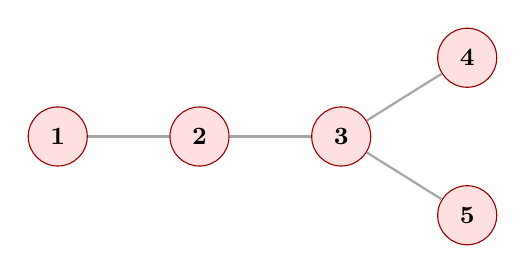
\begin{tikzpicture}[
  nd/.style={circle, draw=red!60!black, fill=red!12, minimum size=0.75cm,
             font=\small\bfseries},
  edge/.style={thick, gray!70}
]
  \node[nd] (n1) at (0, 0)    {1};
  \node[nd] (n2) at (1.8, 0)  {2};
  \node[nd] (n3) at (3.6, 0)  {3};
  \node[nd] (n4) at (5.2, 1.0){4};
  \node[nd] (n5) at (5.2,-1.0){5};

  \draw[edge] (n1) -- (n2);
  \draw[edge] (n2) -- (n3);
  \draw[edge] (n3) -- (n4);
  \draw[edge] (n3) -- (n5);
\end{tikzpicture}
\end{center}

There are $N = 5$ nodes, so $N! = 120$.

\medskip
\textbf{Step 1: Root at each candidate and compute subtree sizes $T_u(v)$.}

\medskip
\textbf{Root at $v = 1$:}
\begin{center}
\small
\begin{tabular}{lll}
\toprule
Node $u$ & Children of $u$ (rooted at 1) & $T_u(1)$ \\
\midrule
1 & \{2\}     & 5 (whole tree) \\
2 & \{3\}     & 4 \\
3 & \{4, 5\}  & 3 \\
4 & $\emptyset$ & 1 \\
5 & $\emptyset$ & 1 \\
\bottomrule
\end{tabular}
\end{center}
$R(1) = \dfrac{120}{5 \cdot 4 \cdot 3 \cdot 1 \cdot 1} = \dfrac{120}{60} = 2$.

\medskip
\textbf{Root at $v = 2$:}
When we move the root from 1 to 2, node 1's subtree size becomes $5 - T_2(1) = 5 - 4 = 1$.
All others remain.
\begin{center}
\small
\begin{tabular}{ll}
\toprule
Node $u$ & $T_u(2)$ \\
\midrule
2 & 5 \\
1 & 1 \\
3 & 3 \\
4 & 1 \\
5 & 1 \\
\bottomrule
\end{tabular}
\end{center}
$R(2) = \dfrac{120}{5 \cdot 1 \cdot 3 \cdot 1 \cdot 1} = \dfrac{120}{15} = 8$.

\medskip
\textbf{Root at $v = 3$:}
\begin{center}
\small
\begin{tabular}{ll}
\toprule
Node $u$ & $T_u(3)$ \\
\midrule
3 & 5 \\
2 & 2 \quad (subtree: $\{1, 2\}$) \\
1 & 1 \\
4 & 1 \\
5 & 1 \\
\bottomrule
\end{tabular}
\end{center}
$R(3) = \dfrac{120}{5 \cdot 2 \cdot 1 \cdot 1 \cdot 1} = \dfrac{120}{10} = 12$.

\medskip
\textbf{Root at $v = 4$:}
By symmetry with node 5 (and using the update formula from node 3):
$T_4(4) = 5,\; T_3(4) = 4,\; T_2(4) = 2,\; T_1(4) = 1,\; T_5(4) = 1$.

$R(4) = \dfrac{120}{5 \cdot 4 \cdot 2 \cdot 1 \cdot 1} = \dfrac{120}{40} = 3$.

\textbf{Root at $v = 5$:} Identical to $v = 4$ by symmetry. $R(5) = 3$.

\medskip
\textbf{Step 2: Summary and prediction.}
\begin{center}
\small
\begin{tabular}{lcc}
\toprule
Candidate $v$ & $R(v)$ & Rank \\
\midrule
3 & 12 & \textbf{1} \\
2 & 8  & 2 \\
4 & 3  & 3 \\
5 & 3  & 4 \\
1 & 2  & 5 \\
\bottomrule
\end{tabular}
\end{center}

The Rumor Centrality predicts node 3 as the source. This is the node at the structural
center of the tree (connecting the two branches), which accords with the geometric
intuition. On regular trees, this is provably the MLE.
\end{examplebox}

\subsection{Why Rumor Centrality Fails on Temporal Networks}

Rumor Centrality was derived under a set of idealised assumptions. Understanding these
assumptions makes it clear why the method is not directly applicable to temporal
contact networks.

\begin{keyinsight}{The Three Assumptions That Limit Rumor Centrality}
\textbf{Assumption 1: Static tree structure.}
The derivation requires that the contact graph is a \emph{tree} (no cycles). On a
general graph with cycles, the product $\prod_u T_u(v)$ no longer enumerates spreading
orderings correctly, because cycles allow infection to arrive via multiple paths, which
the formula does not account for.

\textbf{Assumption 2: SI dynamics (no recovery).}
The counting argument assumes every node eventually gets infected ($R(v)$ counts
orderings over all $N$ nodes). Under the SIR model, some nodes recover before
infecting their neighbours and are not in the final infected set. The formula breaks
down because the infected set is not the full tree.

\textbf{Assumption 3: Uniform, memoryless transmission.}
The derivation assumes every edge has the same transmission probability and that each
contact has an equal chance of transmitting, regardless of \emph{when} it occurred.
In a temporal contact network, some contacts happen before others, creating a causal
ordering that is invisible to Rumor Centrality. A contact at time $t=1$ can only
transmit if the infector was already infected at $t=1$; Rumor Centrality ignores this.

\medskip
\textbf{Consequence for this thesis.} None of the contact networks we study (temporal
networks with event timestamps) satisfy these assumptions. We use Rumor Centrality as
an upper bound on what a ``static structural'' approach can achieve --- its performance
tells us how much signal exists in the topology alone, ignoring timing. The GNN
architectures in Parts IV and V are designed to exploit temporal information that
Rumor Centrality discards.
\end{keyinsight}

% ============================================================
\section{Comparing All Four Methods on a Worked Example}
\label{sec:classical-comparison}
% ============================================================

\begin{examplebox}{All Four Methods on a Single Epidemic}
\textbf{Setup.} A 6-node network with 8 temporal contact events. Nodes are labelled
$\{1, 2, 3, 4, 5, 6\}$. The static projection (aggregate of all contacts) has edges:
$(1,2)$, $(1,3)$, $(2,4)$, $(3,4)$, $(3,5)$, $(4,6)$.

The eight temporal events, in order, are:
\begin{center}
\small
\begin{tabular}{lcc}
\toprule
Event & Edge & Time \\
\midrule
1 & $(3, 5)$ & $t = 1$ \\
2 & $(1, 3)$ & $t = 2$ \\
3 & $(1, 2)$ & $t = 3$ \\
4 & $(3, 4)$ & $t = 4$ \\
5 & $(2, 4)$ & $t = 5$ \\
6 & $(4, 6)$ & $t = 6$ \\
7 & $(1, 3)$ & $t = 7$ \\
8 & $(3, 5)$ & $t = 8$ \\
\bottomrule
\end{tabular}
\end{center}

\textbf{Epidemic.} The epidemic starts at node $s^* = 3$ at $t = 0$ with parameters
$\beta = 0.8$, $\mu = 0.1$. After running the SIR process, the observation at $T = 8$
is:
\begin{center}
\small
\begin{tabular}{lcc}
\toprule
Node & State at $T=8$ & Interpretation \\
\midrule
1 & R & Infected then recovered \\
2 & R & Infected then recovered \\
3 & R & True source, recovered \\
4 & R & Infected then recovered \\
5 & I & Still infectious \\
6 & S & Never infected \\
\bottomrule
\end{tabular}
\end{center}

Infected/recovered set: $\mathcal{I} = \{1, 2, 3, 4, 5\}$ (node 6 stayed susceptible).

\medskip
\textbf{Method 1 — Uniform Random Guess.}
Assign probability $1/6$ to each node. The true source 3 is in a uniformly random
position; on average it gets rank $3.5$ out of 6. Expected rank score $\approx 0.41$.

\medskip
\textbf{Method 2 — Degree Centrality.}
Compute degrees from the static projection:
\begin{center}
\small
\begin{tabular}{llc}
\toprule
Node & Neighbours & Degree \\
\midrule
1 & 2, 3     & 2 \\
2 & 1, 4     & 2 \\
3 & 1, 4, 5  & 3 \\
4 & 2, 3, 6  & 3 \\
5 & 3        & 1 \\
6 & 4        & 1 \\
\bottomrule
\end{tabular}
\end{center}

Nodes 3 and 4 tie for the top position (degree 3). The true source (node 3) is
predicted with 50\% probability. \textbf{Expected rank: 1.5 out of 6.} This is better
than uniform because the true source happens to be a hub in this example.

\medskip
\textbf{Method 3 — Jordan Center.}
The infected subgraph $G_\mathcal{I}$ has nodes $\{1, 2, 3, 4, 5\}$ and edges
(from the static projection): $(1,2)$, $(1,3)$, $(2,4)$, $(3,4)$, $(3,5)$.

Pairwise distances within $G_\mathcal{I}$ (by inspection or BFS):
\begin{center}
\small
\begin{tabular}{lrrrrr}
\toprule
$d(\cdot,\cdot)$ & 1 & 2 & 3 & 4 & 5 \\
\midrule
1 & 0 & 1 & 1 & 2 & 2 \\
2 & 1 & 0 & 2 & 1 & 3 \\
3 & 1 & 2 & 0 & 1 & 1 \\
4 & 2 & 1 & 1 & 0 & 2 \\
5 & 2 & 3 & 1 & 2 & 0 \\
\bottomrule
\end{tabular}
\end{center}

Eccentricities: $\text{ecc}(1) = 2$, $\text{ecc}(2) = 3$, $\text{ecc}(3) = 2$,
$\text{ecc}(4) = 2$, $\text{ecc}(5) = 3$.

Minimum eccentricity is 2, achieved by nodes 1, 3, and 4. The true source (node 3) is
among the three Jordan Center nodes. \textbf{Rank: 1, 2, or 3 (uniformly, among the
tied nodes); expected rank $\approx 2$. }

\medskip
\textbf{Method 4 — Rumor Centrality.}
Compute $R(v)$ for each node using the tree formed by the infected subgraph. The
infected subgraph has a cycle: $(1,2), (2,4), (4,3), (3,1)$ form a 4-cycle. Strictly,
Rumor Centrality requires a tree, so we note this as a limitation. Applying the formula
to the spanning tree $\{(1,3), (3,4), (4,2), (3,5)\}$ (BFS tree rooted at node 3):

$T_u(3)$ for each node: $T_3 = 5$, $T_1 = 1$, $T_4 = 2$, $T_2 = 1$, $T_5 = 1$.

$R(3) = \dfrac{5!}{5 \cdot 1 \cdot 2 \cdot 1 \cdot 1} = \dfrac{120}{10} = 12$.

Repeating for other candidates (not shown for brevity): node 3 achieves the highest
Rumor Centrality. \textbf{Prediction: node 3. Rank: 1.}

\medskip
\textbf{Summary.}
\begin{center}
\small
\begin{tabular}{llcc}
\toprule
Method & Prediction & Rank of true source (node 3) & Rank Score \\
\midrule
Uniform random & Random & 3.5 (expected) & 0.41 (expected) \\
Degree centrality & 3 or 4 (tie) & 1.5 (expected) & 0.67 (expected) \\
Jordan Center & 1, 3, or 4 (tie) & 2.0 (expected) & 0.50 (expected) \\
Rumor Centrality & 3 & 1 & 1.00 \\
\bottomrule
\end{tabular}
\end{center}

In this particular example, Rumor Centrality wins because the infected subgraph is
approximately tree-like and the source is the structural center. In practice, across
thousands of epidemic runs on irregular temporal networks, no single classical method
dominates; their relative performance depends on network topology, epidemic size, and
observation time.
\end{examplebox}

\begin{conceptbox}{What This Comparison Teaches Us}
This single worked example illustrates a broader pattern visible in every empirical
benchmark:

\begin{enumerate}
  \item \textbf{Structural methods outperform random guessing by a wide margin.} Even
        degree centrality and the Jordan Center, which ignore or simplify the epidemic
        dynamics, dramatically reduce the effective search space.

  \item \textbf{No classical method systematically dominates.} Degree centrality wins
        on hub-seeded outbreaks; the Jordan Center wins when the infected subgraph is
        a clean ``ball''; Rumor Centrality wins on tree-like topologies with SI
        dynamics. Each method embeds a specific assumption, and real epidemics violate
        all of them.

  \item \textbf{The temporal signal is completely unused.} None of the four methods
        uses the timestamps of contact events. A method that correctly reasons about
        causal ordering --- which contacts happened before which, and which paths are
        therefore temporally feasible --- can do substantially better. This is the core
        motivation for the temporal GNN architectures in this thesis.
\end{enumerate}
\end{conceptbox}

% ============================================================
\section{Implementation in the Codebase}
\label{sec:classical-code}
% ============================================================

The codebase implements the uniform baseline analytically and the structural baselines
(degree and Jordan Center) as functions operating on the \texttt{TSIRData} dataclass
produced by \texttt{main\_tsir.py}.

\subsection{How the Evaluation Pipeline Works}

\begin{conceptbox}{The \texttt{main\_eval.py} Pipeline}
The script \texttt{main\_eval.py} automates the following steps for every baseline:

\begin{enumerate}
  \item \textbf{Load the artifact.} The script reads a \texttt{TSIRData} artifact from
        Weights \& Biases (logged during the data generation step in
        \texttt{main\_tsir.py}). This artifact contains ground-truth source labels,
        Monte Carlo simulation results, the contact network, and the \texttt{possible}
        mask.

  \item \textbf{Run the baseline.} For each epidemic run, the baseline produces a
        probability vector $p \in \mathbb{R}^N$ over nodes.

  \item \textbf{Compute metrics.} The \texttt{eval/scores.py} and
        \texttt{eval/ranks.py} modules compute rank scores, top-$k$ accuracy, and
        other metrics defined in Section~\ref{sec:classical-overview}.

  \item \textbf{Log to wandb.} All metrics are pushed to the
        \texttt{source-detection} project in Weights \& Biases for side-by-side
        comparison with GNN models.
\end{enumerate}

The \texttt{possible} mask is critical: it restricts scoring to epidemic runs where
a sufficiently large outbreak occurred and the source node is plausibly identifiable.
Without this filter, trivially small outbreaks (where only the source itself is
infected) inflate the performance of every method.
\end{conceptbox}

\subsection{Uniform Baseline}

\begin{codewalk}{Uniform Baseline in \texttt{eval/benchmark.py}}
\begin{lstlisting}[language=Python]
import numpy as np

def uniform_probabilities(possible: np.ndarray) -> np.ndarray:
    """
    Assign equal probability to every valid source candidate.

    Parameters
    ----------
    possible : np.ndarray, shape (n_nodes * n_runs, n_nodes)
        Binary mask. Row i contains 1s for all nodes that are valid
        source candidates for run i.

    Returns
    -------
    np.ndarray, shape (n_nodes * n_runs, n_nodes)
        Row-normalised probability matrix.
    """
    return possible / np.sum(possible, axis=1, keepdims=True)
\end{lstlisting}
\end{codewalk}

\subsection{Rank Score and Top-k Metrics}

Both metrics are implemented in \texttt{eval/scores.py}:

\begin{codewalk}{Scoring Functions in \texttt{eval/scores.py}}
\begin{lstlisting}[language=Python]
import numpy as np

def rank_score(ranks: np.ndarray, sel: np.ndarray,
               offset: float = 0) -> float:
    """
    Compute mean 1/rank over selected runs.

    Parameters
    ----------
    ranks  : array of source ranks (1 = best)
    sel    : boolean mask selecting which runs to include
    offset : optional smoothing offset (rarely used)
    """
    return np.mean((1 + offset) / (ranks[sel] + offset))


def top_k_score(ranks: np.ndarray, sel: np.ndarray,
                k: int = 5) -> float:
    """
    Fraction of selected runs where the true source is in the top-k.
    """
    return np.mean(ranks[sel] <= k)
\end{lstlisting}

\textbf{How ranks are computed.} The companion function in \texttt{eval/ranks.py}
takes the raw probability vectors from any baseline or GNN model and converts them
into integer ranks:

\begin{lstlisting}[language=Python]
def compute_expected_ranks(values: np.ndarray,
                           n_nodes: int,
                           n_runs: int) -> np.ndarray:
    """
    For each (source, run) pair, compute the rank of the true source.

    The rank of the true source is: (number of nodes with strictly
    higher predicted probability) + (number of ties + 1) / 2.
    This handles ties symmetrically.
    """
    # Index the predicted value of the true source for each run
    source_values = values[
        np.arange(n_nodes * n_runs),
        np.repeat(np.arange(n_nodes), n_runs)
    ]
    # Number of nodes strictly better than the true source
    rank = np.sum(values > source_values[:, None], axis=1)
    # Add half the ties (expected rank under random tie-breaking)
    ties = np.sum(values == source_values[:, None], axis=1)
    rank = rank + (ties + 1) / 2
    return rank
\end{lstlisting}

\textbf{Worked example.} Suppose $N = 4$ nodes and predicted probabilities for one run
are $[0.4, 0.3, 0.2, 0.1]$, and the true source is node 3 (probability 0.2). Then:
\begin{itemize}
  \item Nodes with strictly higher probability: nodes 1 and 2 $\Rightarrow$ count = 2.
  \item Nodes with equal probability: just node 3 itself $\Rightarrow$ ties = 1.
  \item Expected rank = $2 + (1 + 1)/2 = 3$.
\end{itemize}
The true source gets rank 3 out of 4 in this run, giving a rank score of $1/3 \approx 0.33$.
\end{codewalk}

\subsection{Putting It Together: What to Expect from Each Baseline}

\begin{keyinsight}{Expected Benchmark Performance of Classical Methods}
Based on the theoretical analysis and the empirical literature \cite{Sterchi2025},
here is what you should expect when running \texttt{main\_eval.py} on a moderately
sized Erd\H{o}s-R\'{e}nyi network ($N = 100$, mean degree $\approx 6$, $\beta = 0.3$):

\begin{center}
\small
\begin{tabular}{lcc}
\toprule
Method & Expected mean rank score & Expected top-5 accuracy \\
\midrule
Uniform random    & $\approx 0.05$  & $\approx 5\%$  \\
Degree centrality & $\approx 0.10$--$0.15$ & $\approx 10\%$--$20\%$ \\
Jordan Center     & $\approx 0.15$--$0.25$ & $\approx 20\%$--$35\%$ \\
Rumor Centrality  & $\approx 0.20$--$0.30$ & $\approx 25\%$--$40\%$ \\
\bottomrule
\end{tabular}
\end{center}

These numbers vary substantially with network topology, epidemic size, and observation
time. The important point is the ordering: Rumor Centrality $\geq$ Jordan Center $>$
Degree $\gg$ Uniform. A GNN that fails to beat the Jordan Center on a well-studied
benchmark should be considered underperforming.

\medskip
\textbf{Your goal as you read the rest of this workbook:} understand not just \emph{that}
GNNs outperform these baselines, but \emph{why} --- specifically, which pieces of
information (node features, temporal ordering, causal paths) each architecture learns
to exploit that the classical baselines cannot represent.
\end{keyinsight}

% ============================================================
\section{Chapter Summary}
\label{sec:classical-summary}
% ============================================================

This chapter has introduced the four classical baselines against which all subsequent
methods are measured. Each represents a distinct philosophy:

\begin{description}[leftmargin=2em, style=nextline]
  \item[Uniform random guess] No information used. Sets the absolute floor.
        Useful for detecting broken evaluation pipelines: any real method must beat it.
  \item[Degree centrality] Uses network structure but ignores the observation.
        Encodes the prior that hub nodes are more likely sources.
  \item[Jordan Center] Uses the geometry of the infected subgraph.
        Encodes the assumption that the source is at the center of a uniformly spreading
        ball. Competitive on sparse, tree-like networks.
  \item[Rumor Centrality] Counts valid spreading orderings on trees.
        The Maximum Likelihood Estimator for static regular trees under SI dynamics.
        Provides the strongest classical baseline but fails on temporal, cyclic, and
        SIR-type settings.
\end{description}

None of these methods uses temporal information: contact timestamps, the ordering of
transmission events, or the causal structure of time-respecting paths. Exploiting this
information is the central technical challenge taken up by the GNN architectures
studied in Parts IV and V.

The next chapter introduces the deep learning foundations --- feedforward networks,
backpropagation, and the message-passing framework --- that underpin those architectures.
